\documentclass[10pt]{beamer}
\usetheme[progressbar=frametitle]{metropolis}

\usepackage [autostyle, english = american]{csquotes}
\DeclareFontShape{OT1}{cmss}{b}{n}{<->ssub * cmss/bx/n}{} 
\usepackage{amsmath}
\usepackage{amssymb}
\usepackage{bm} 
\usepackage{multicol}

\MakeOuterQuote{"}
\newcommand{\imp}[1]{\textbf{\color{cyan}#1}}

%---------------------------------------------------
% Title 

\title{Refining Character Relationships in a Textual Narrative using Embeddings of Interactions}
\subtitle{With case studies on \emph{Les Misérables}}
\date{}
\author{Guillaume Guex}
\institute{University of Lausanne}

\begin{document}
	
	%------------------------------------------------------------------
	
	\maketitle
	
	%------------------------------------------------------------------
	
	\begin{frame}{Table of contents}
		\setbeamertemplate{section in toc}[sections numbered]
		\tableofcontents%[hideallsubsections]
	\end{frame}

	%------------------------------------------------------------------
	
	\section[Introduction]{Introduction}
	
	%------------------------------------------------------------------
	
	\begin{frame}{The construction of a character network}
		The construction of a character network takes generally 3 steps \cite{labatut_extraction_2019}:
		\begin{itemize}
			\item Identification of \imp{characters} 
			\item Detection of \imp{interactions}
			\item Construction of the \imp{graph}
		\end{itemize}
	\end{frame}

	%------------------------------------------------------------------
	
	\begin{frame}{The construction of a character network}
		When dealing with \imp{textual narratives}, a frequently used method is to count \imp{character co-occurrences} in predefined \imp{textual units} \\(see, e.g., \cite{elsner_character-based_2012, rochat_analyse_2014}). \\
		\vspace{-0.4cm}
		\begin{columns}
			\begin{column}{0.5\textwidth}
				\begin{figure}
					\centering
					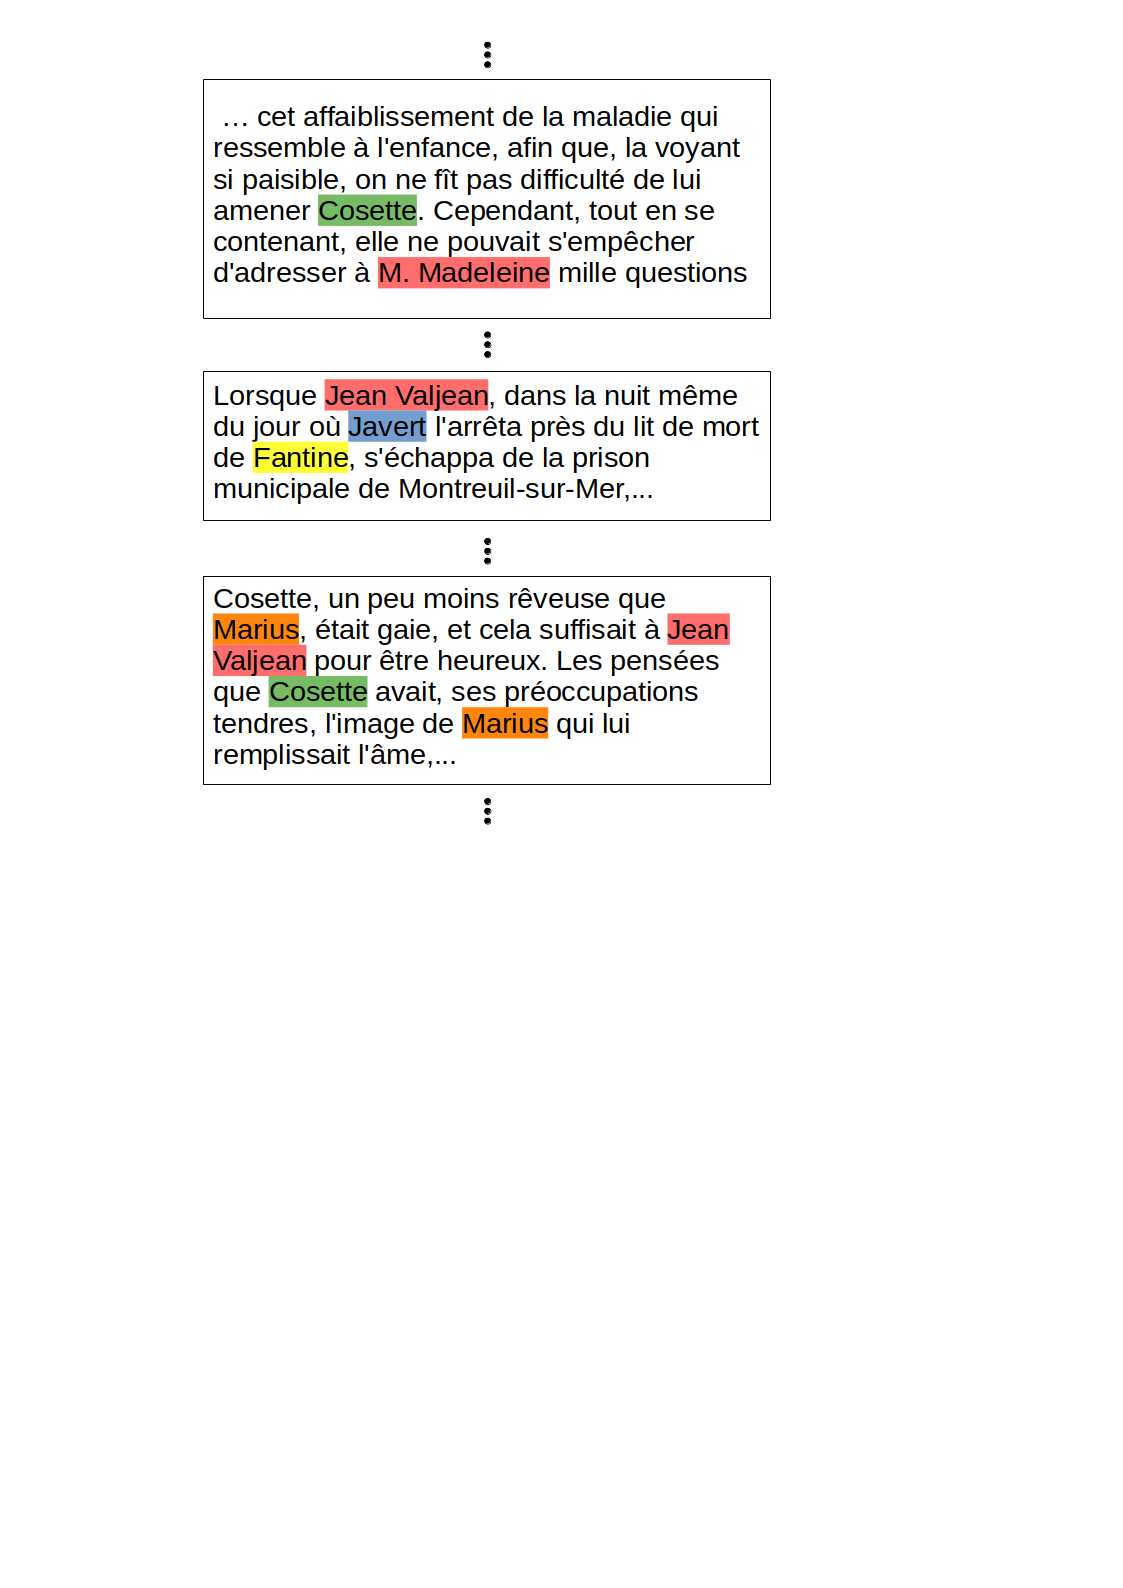
\includegraphics[width=1.4\textwidth]{img/textual_units.png}
				\end{figure}
			\end{column}
			\begin{column}{0.5\textwidth}
				\vspace{-4cm}
				\begin{table}
					\centering
					\scriptsize
					\begin{tabular}{|c|c|c|} 
						\hline
						Character 1 & Character 2 & Co-occurrences \\ 
						\hline
						Cosette & Marius & 1 \\
						Cosette & Valjean & 2 \\ 
						Fantine & Javert & 1 \\
						Fantine & Valjean & 1 \\
						Javert & Valjean & 1 \\
						Marius & Valjean & 1 \\
						\hline
					\end{tabular}
				\end{table}
				\begin{figure}
					\centering
					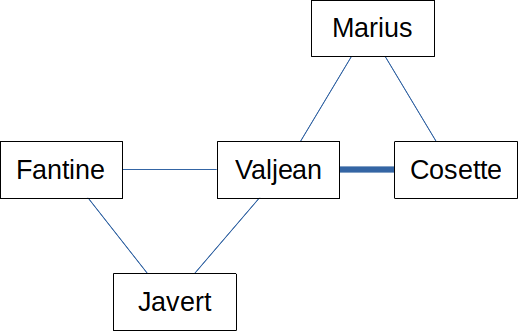
\includegraphics[width=0.8\textwidth]{img/mini_graph.png}
				\end{figure}
			\end{column}
		\end{columns}
	\end{frame}
	
	%------------------------------------------------------------------
	
	\begin{frame}{Dataset}
		In this context, the \imp{dataset} used to construct the character network has the following form
		\begin{figure}
			\centering
			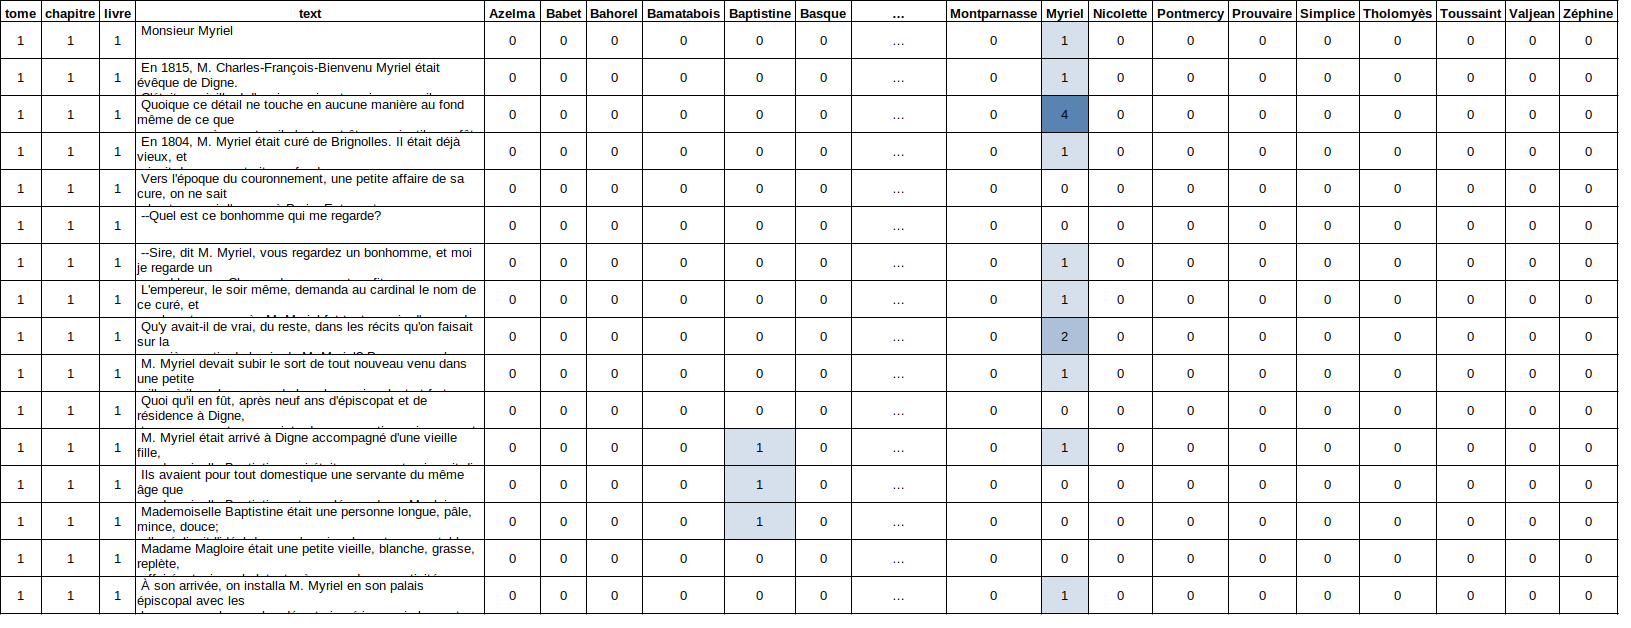
\includegraphics[width=\textwidth]{img/data_table.png}
		\end{figure}
		However, apart from a few exceptions \cite{nalisnick_character--character_2013, trovati_towards_2014, min_modeling_2019}, the content of the \imp{text column} is not used. \imp{Edges in the resulting graph aggregate blindly various kind of interactions}.
	\end{frame}
	
	
	%------------------------------------------------------------------
	
	\begin{frame}{Approaches}
		In this presentation, we propose to \imp{refine character relationships} by using the \imp{textual data}. Quantities of approaches can be undertaken, but we focus on:
		\begin{itemize}
			\item \imp{Bag-of-paths} approaches, a corpus is represented by an \imp{unit-term matrix}. \\
			\vspace{0.3cm}
			\begin{figure}
				\centering
				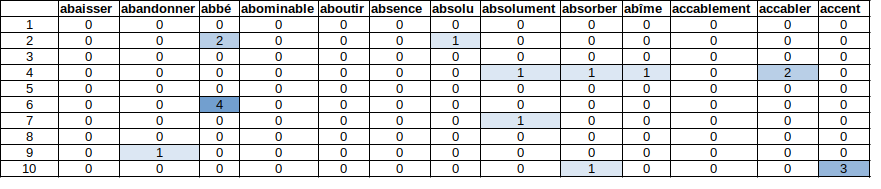
\includegraphics[width=0.8\textwidth]{img/unit_term.png}
			\end{figure}
			\item \imp{Embeddings of textual units}. The unit-term matrix is used to construct \imp{vectors} representing units. 
			\item \imp{Embeddings of characters and relationships}, which derive from the embedding of textual units.
		\end{itemize}
	\end{frame}
	
	
	%------------------------------------------------------------------
	
	\begin{frame}{Approaches}
		More specifically, two types "embeddings" are studied:
		\begin{itemize}
			\item \imp{Correspondence Analysis (CA)}.
			\item \imp{"Topic Modeling vectors"} build from \imp{Non-negative Matrix Factorization (NMF)}.
		\end{itemize}
		With two methods for constructing character/relationship vectors:
		\begin{itemize}
			\item \imp{Centroids}.
			\item \imp{Regression coefficients}.
		\end{itemize}
	\end{frame}
	
	
	%------------------------------------------------------------------
	
	
	\section[Correspondence Analysis (CA) - centroids]{Correspondence Analysis (CA) - centroids}
	
	%------------------------------------------------------------------
	
	\begin{frame}{Principles}
		Correspondence Analysis is the natural tool for analyzing textual resources if data are organized in a $(n \times p)$ \imp{document-term matrix} \cite{lebart_analyse_2019} (here, documents are our textual units). It gives:
		\begin{itemize}
			\item $\min(n, p) - 1$ \imp{factorial axes}, by decreasing order of importance, which can be interpreted as latent variables.
			\item \imp{Coordinates of each document} along these factors, where proximity can be interpreted as similar profile in term of words.
			\item \imp{Coordinates of each word} along the same factors, where proximity can be interpreted as similar profile in term of documents.
			\item \imp{Affinities between a document and a term}, which is computed by the \imp{scalar product} between their vectors.
		\end{itemize}
	\end{frame}
	
	%------------------------------------------------------------------
	
	\begin{frame}{Principles}
		If we plot units and words on the first two axes, we get the usual \imp{biplot}:
		\begin{figure}
			\centering
			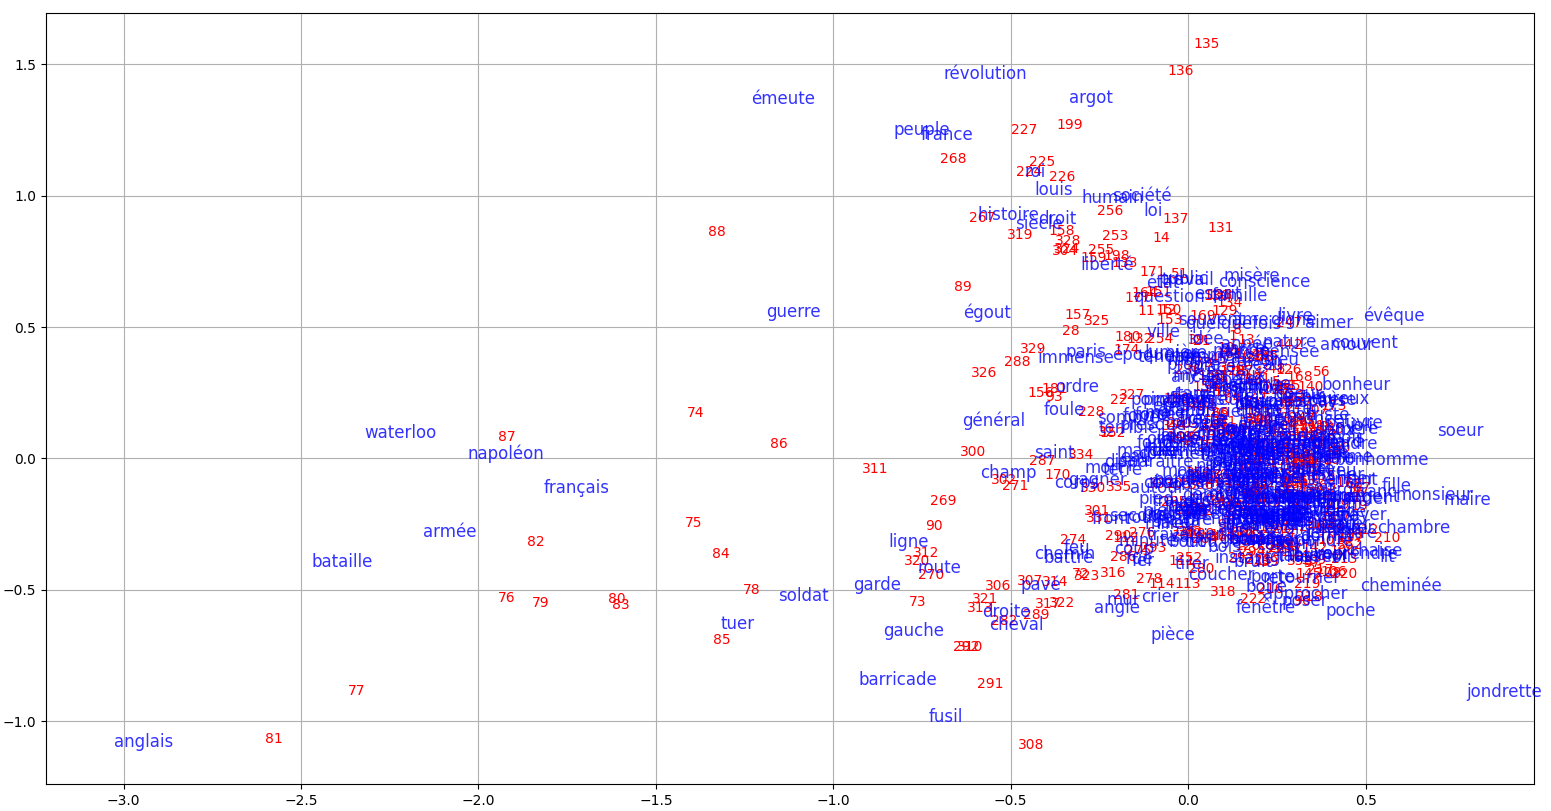
\includegraphics[width=\textwidth]{img/biplot.png}
		\end{figure}
	\end{frame}
	
	%------------------------------------------------------------------
	
	\begin{frame}{Characters embeddings - centroids}
		The \imp{textual units} have natural embedding in CA. For characters, the most intuitive idea is to compute them as \imp{centroids} of units where they appear.
		\begin{figure}
			\centering
			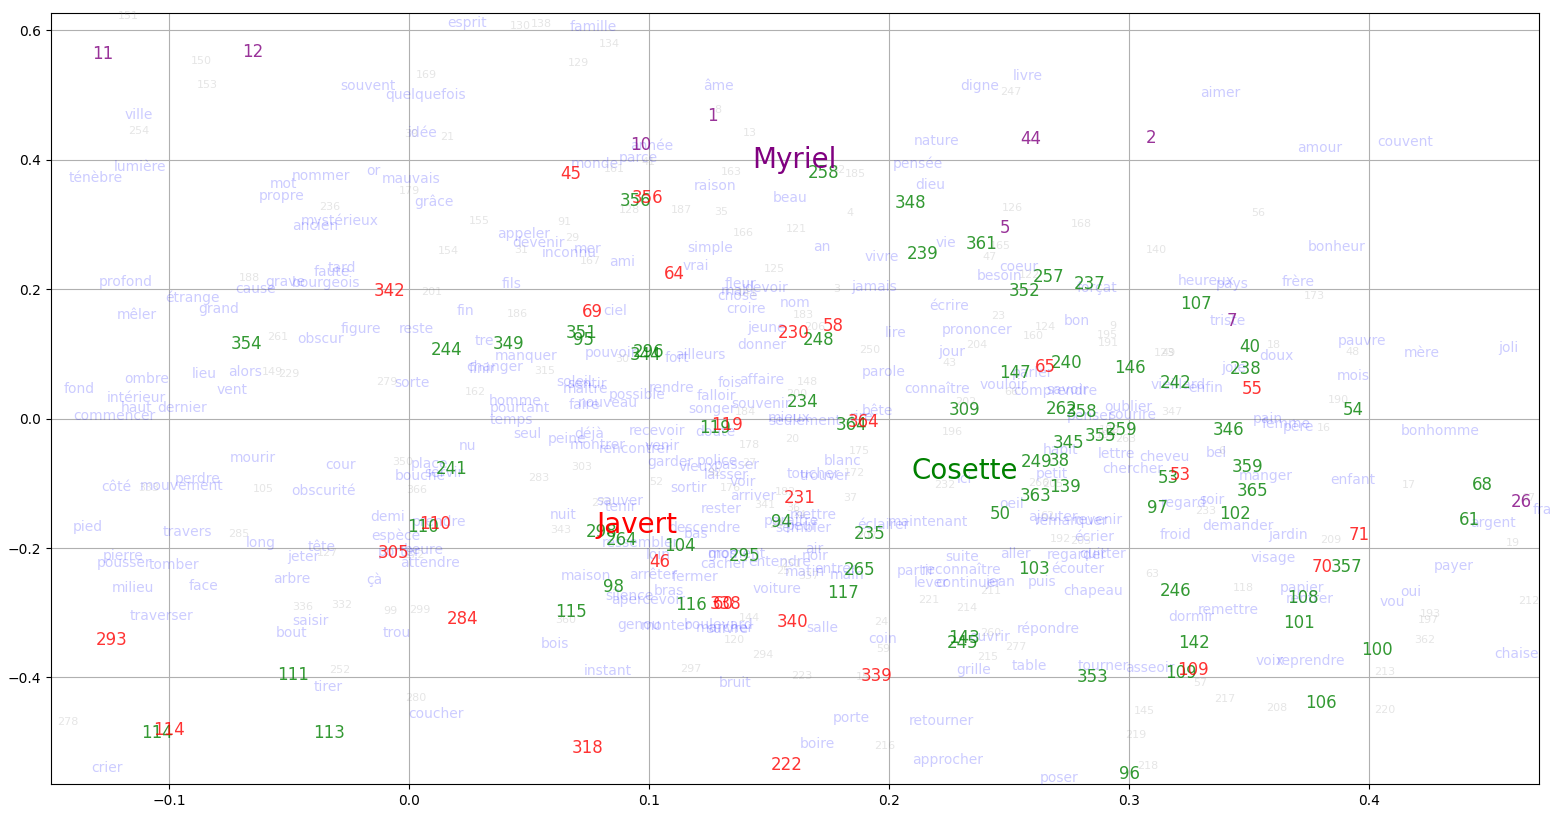
\includegraphics[width=\textwidth]{img/char_embeddings.png}
		\end{figure}
	\end{frame}
	
	%------------------------------------------------------------------
	
	\begin{frame}{Relationship embeddings - centroids}
		The same idea can be applied to \imp{relationships}, In fact, in our data table, we can extend our table to include \imp{interactions}.
		\begin{figure}
			\centering
			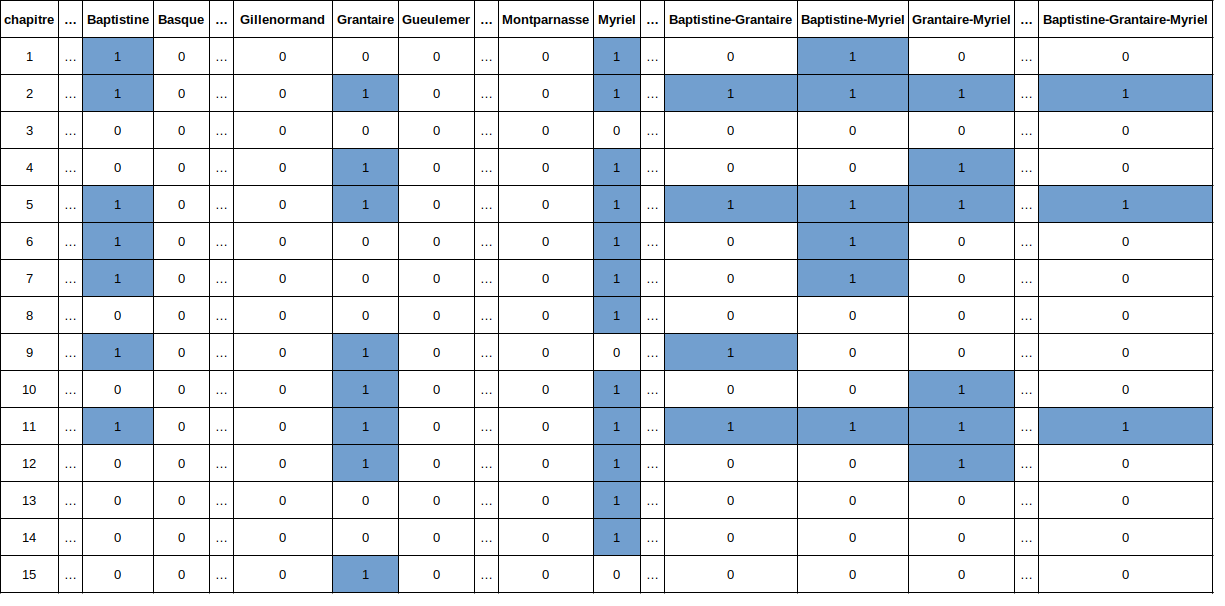
\includegraphics[width=\textwidth]{img/occurences_data.png}
		\end{figure}
	\end{frame}
	
	%------------------------------------------------------------------
	
	\begin{frame}{Relationship embeddings - centroids}
		This leads us with embeddings of \imp{relationships}:
		\begin{figure}
			\centering
			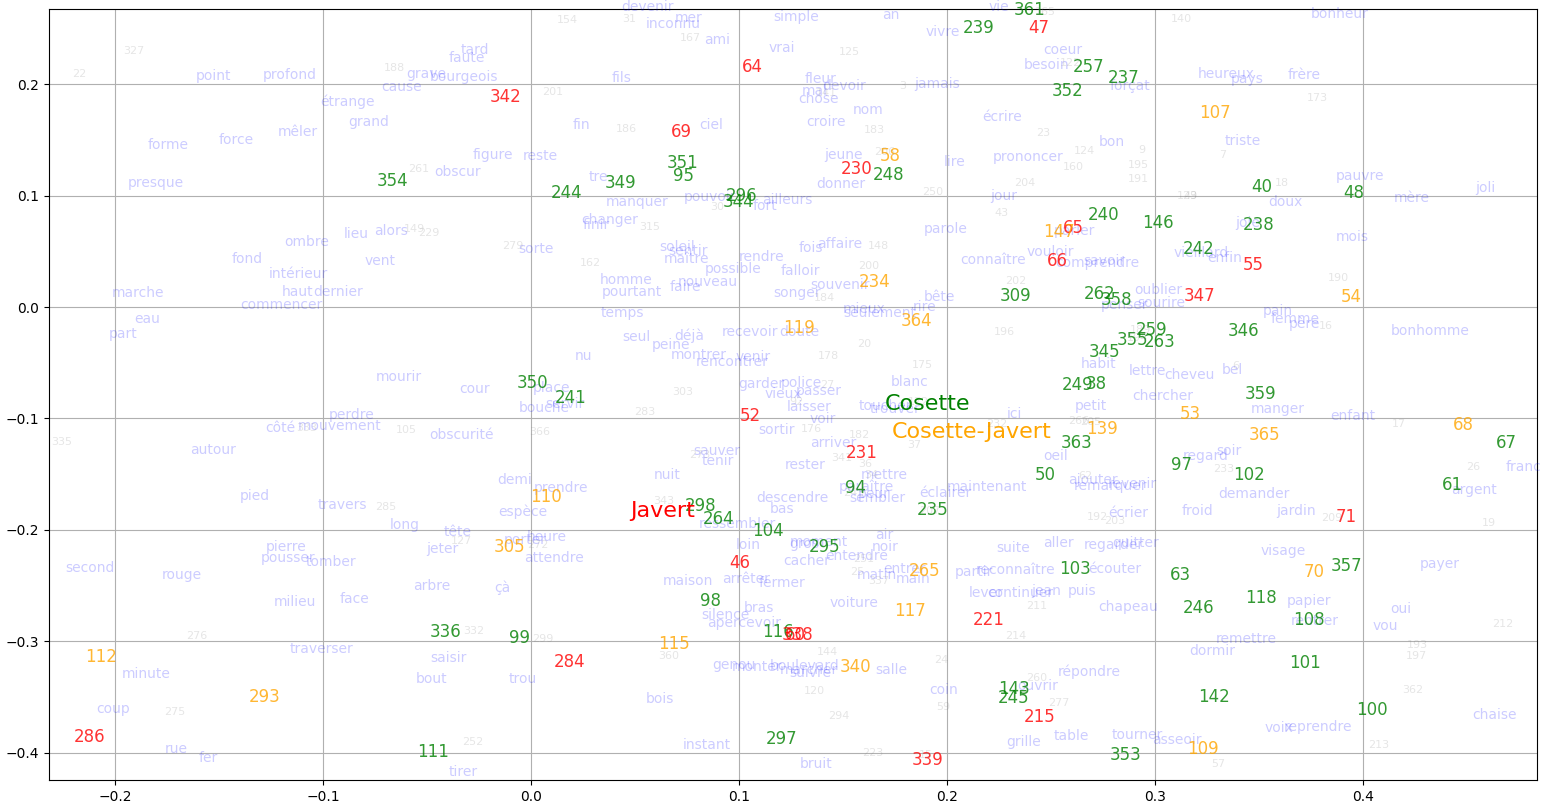
\includegraphics[width=\textwidth]{img/occ_embeddings.png}
		\end{figure}
	\end{frame}
	
	%------------------------------------------------------------------
	
	\begin{frame}{Character/relationship embeddings - usages}
		What can we do with these character/relationship embeddings ? As they are in the same space as textual units, we can: 
		\begin{itemize}
			\item Get the Euclidean distance between \imp{relationships}.
			\item Get the Euclidean distance between \imp{relationships and the textual units}.
			\item Observe their values on the different \imp{factorial axes}. 
			\item Observe similarities (scalar product) between \imp{relationships and words (or group of words)}.
		\end{itemize}
	\end{frame}
	
	%------------------------------------------------------------------
	
	\begin{frame}{Characters/relationships vs axes}
		Sometimes, \imp{factorial axes can be interpreted with coordinates of the words}. \imp{Positions of characters/relationships on this axis} reflect their affinity with this particular scale:
		\begin{figure}
			\centering
			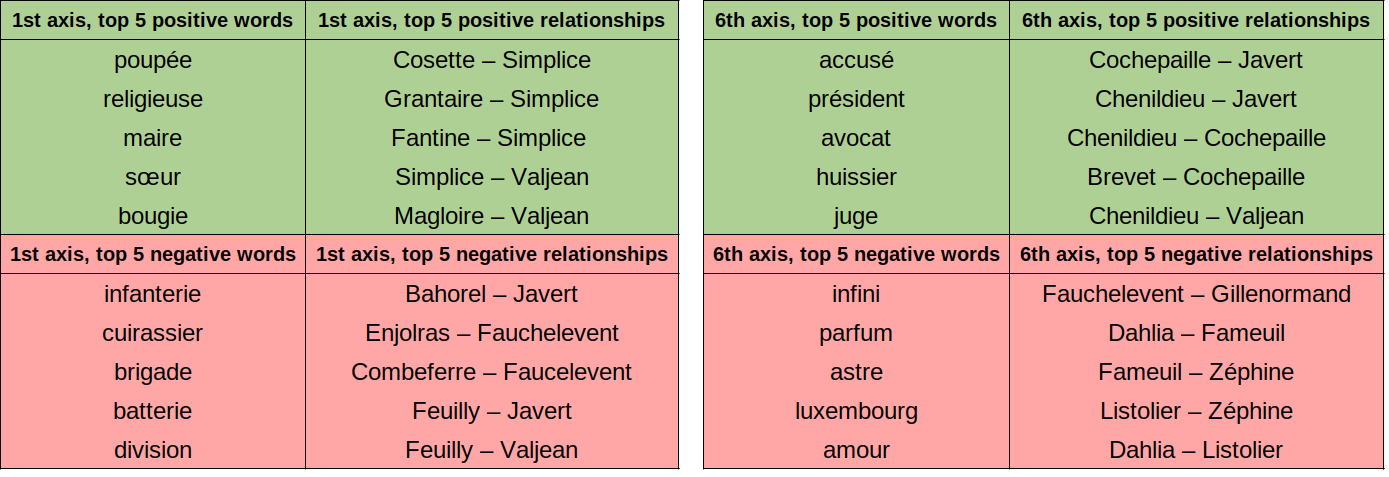
\includegraphics[width=\textwidth]{img/relationship_vs_axes.png}
		\end{figure}
	\end{frame}
	
	%------------------------------------------------------------------
	
	\begin{frame}{Characters/relationships vs words}
		We can also get the \imp{similarities between characters/relationships vs words} with the help of the \imp{scalar product}:
		\begin{figure}
			\centering
			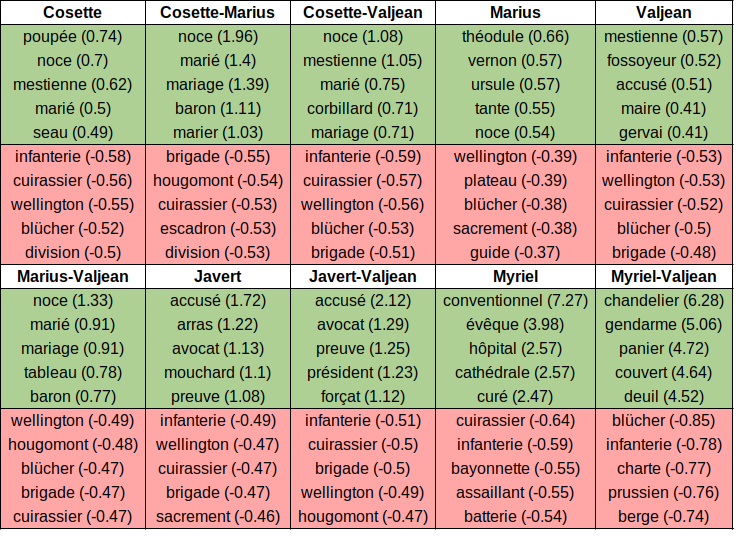
\includegraphics[width=0.8\textwidth]{img/relationships_vs_words.png}
		\end{figure}
	\end{frame}
	
	%------------------------------------------------------------------
	
	\begin{frame}{Words vs characters/relationships}
		By transposing the previous table, particular words (or group of words, i.e. a query) can give a ranking of characters/relationships:
		\begin{figure}
			\centering
			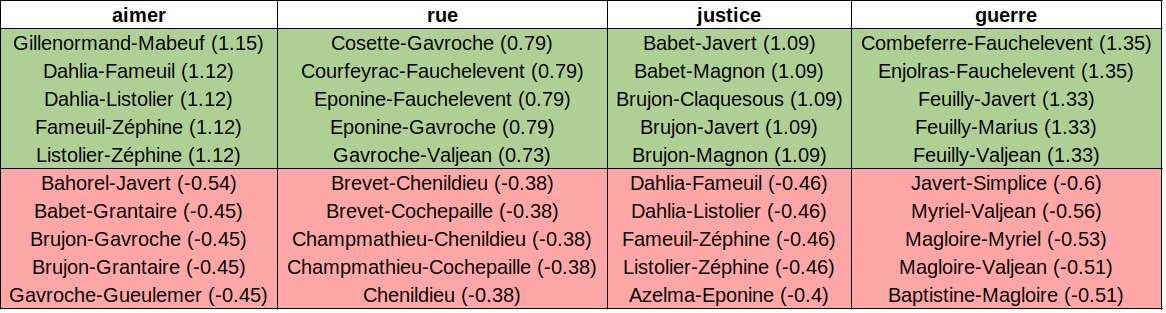
\includegraphics[width=\textwidth]{img/word_vs_occ.png}
		\end{figure}
		In this case, the centroid method seems to show its limit.
	\end{frame}
	
	%------------------------------------------------------------------
	
	
	\section[Correspondence Analysis (CA) - regressions]{Correspondence Analysis (CA) - regressions}
	
	%------------------------------------------------------------------
	
	\begin{frame}{Relationship embeddings - 1st idea problems}
		In fact, building these character/relationship vectors as \imp{centroids} is like considering them as \imp{additional variables} in the CA. It leads to \imp{additive relationships}, i.e., for a character $c$
		$$
		v_{c} = \sum_{d \in \text{characters}} v_{cd}
		$$
		where $v_{cd}$ is the vector of relationship between $c$ and $d$, and $v_{cc}$ is defined as the centroid of units where $c$ is alone. This means
		\begin{itemize}
			\item If a character have \imp{contrasted relationships}, its vector might represent it poorly.
			\item If \imp{two characters are often together}, their respective specificities might be hidden.
			\item If \imp{two relationships are often together}, their respective specificities might be hidden.
		\end{itemize}
		\emph{Are we the sum of our relationships (+ ourself alone)?} 
	\end{frame}
	
	%------------------------------------------------------------------
	
	\begin{frame}{Relationship embeddings - 2nd idea}
		A way to avoid this problem, is to consider that
		\begin{itemize}
			\item The appearance of character \imp{$c$ alone} gives a particular profile to units.
			\item The appearance of character \imp{$d$ alone} gives another profile to units.
			\item The appearance of character \imp{$c$ and $d$} might give a totally \imp{different profile} to units.
		\end{itemize}
		We can use a \imp{regression model with interaction}.
	\end{frame}
	
	%------------------------------------------------------------------
	
	\begin{frame}{Relationship embeddings - 2nd idea}
		Let $(y_1, \ldots, y_n)$ be the coordinates of the $n$ units on the \imp{first factorial axis}, $\delta(c)$ the indicator variable of character $c$ presence, and $\delta(c,d)$ the indicator variable of relationship $c,d$ presence. We can fit the model:
		$$
		\hat{y} = \beta_0 + \sum_{c} \beta_c \delta(c) + \sum_{c,d} \beta_{cd} \delta(c,d)
		$$
		with a \imp{Ridge (L2) regularization term}, parameterized by $\lambda$, to avoid overfitting.
		\begin{itemize}
		\item The first coordinate of a \imp{character-vector $c$ is given by $\beta_c$}.
		\item The first coordinate of a \imp{relationship-vector $(c,d)$ is given by $\beta_{cd}$}.
		\end{itemize}
		We do a \imp{similar regression on all axis to get vectors}.
	\end{frame}
	
	%------------------------------------------------------------------
	
	\begin{frame}{Relationship embeddings - 2nd idea}
		Resulting coordinates of opposite characters point at \imp{different directions}:
		\begin{figure}
			\centering
			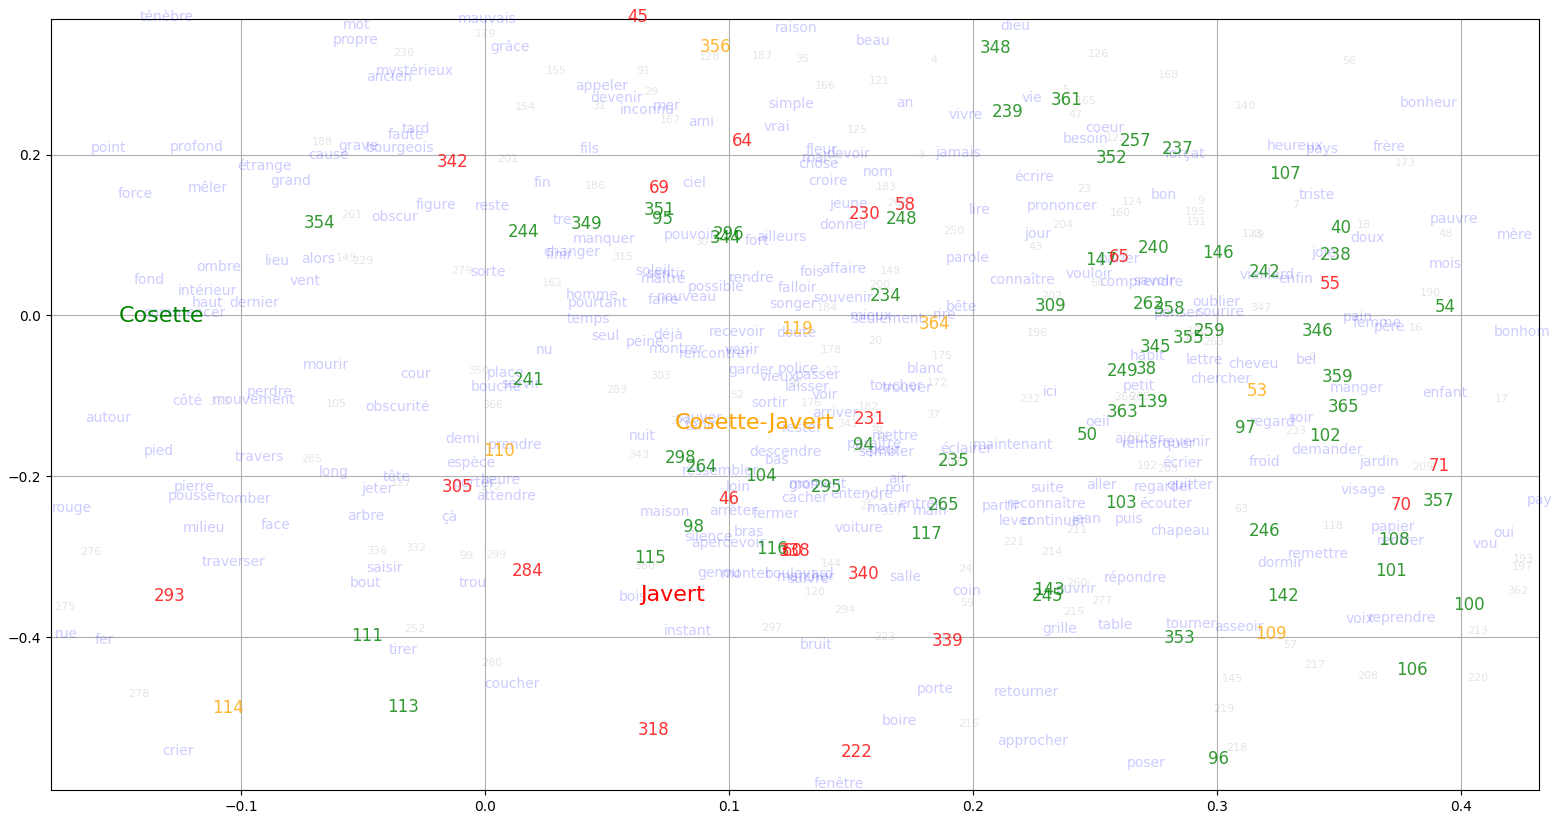
\includegraphics[width=\textwidth]{img/reg_embeddings.png}
		\end{figure}
	\end{frame}
	
	%------------------------------------------------------------------
	
	\begin{frame}{Relationship embeddings - 2nd idea}
		The \imp{regularizing parameter $\lambda$} has an interesting effect on resulting vectors:
		\begin{itemize}
			\item When $\lambda$ is \imp{high}, the \imp{vectors are similar to centroids} (with a different scaling).
			\item When $\lambda$ is \imp{low}, the solution focuses on \imp{very specific, small parts of the text} to define characters and relationships.
			\item An \imp{average} $\lambda$ (but which one?) is able to \imp{highlight character/relationship specificities relatively to corpus size.}
		\end{itemize}
	\end{frame}
	
	%------------------------------------------------------------------
	
	\begin{frame}{Characters/relationships vs words - comparisons}
		With regressions, there is more \imp{variety} in words defining characters/relationships:
		\vspace{-0.2cm}
		\begin{figure}
			\centering
			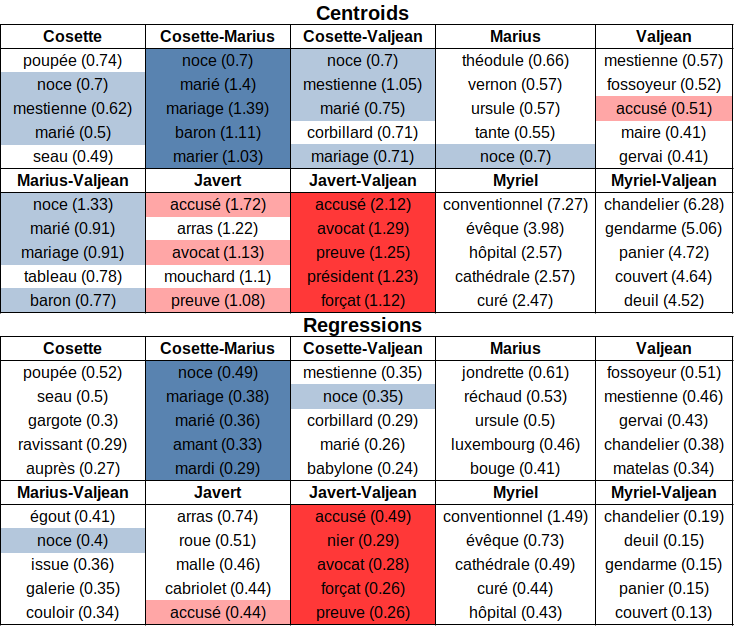
\includegraphics[width=0.7\textwidth]{img/reg_vs_word.png}
		\end{figure}
	\end{frame}
	
	%------------------------------------------------------------------
	
	\begin{frame}{Words vs characters/relationships - regression}
		And relationships according to words are more coherent:
		\vspace{-0.2cm}
		\begin{figure}
			\centering
			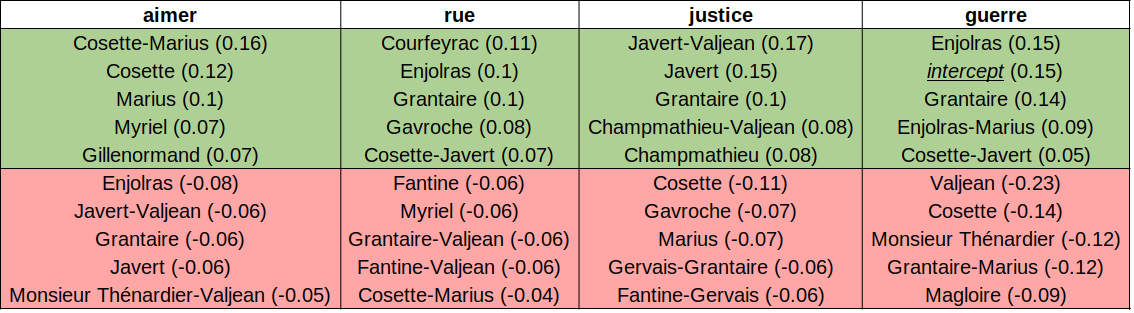
\includegraphics[width=\textwidth]{img/word_vs_reg.png}
		\end{figure}
	\end{frame}
	
	%------------------------------------------------------------------
	
	\begin{frame}{Words vs characters/relationships - regression}
		This method give also good results if regressors are constructed according to a \imp{narrative timeline} (here, the \emph{Tomes}):
		\vspace{-0.2cm}
		\begin{figure}
			\centering
			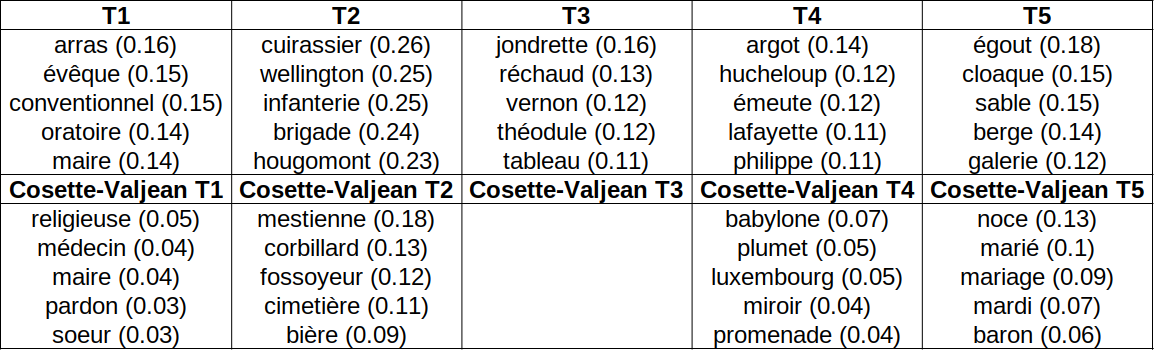
\includegraphics[width=\textwidth]{img/reg_vs_word_long.png}
		\end{figure}
	\end{frame}
	
	%------------------------------------------------------------------
	
	\begin{frame}{CA quick summary}
		To recap the CA method:
		\begin{itemize}
			\item \imp{Words and units vectors} are obtained from the \imp{unit-term matrix}.
			\item \imp{Characters/Relationships vectors} are obtained with 2 different methods:
			\begin{itemize}
				\item \imp{Centroids}
				\item \imp{Regressions}
			\end{itemize}
			\item These characters/relationships vectors can be \imp{explored} regarding:
			\begin{itemize}
				\item \imp{Axes}
				\item \imp{Words} (or group of words)
			\end{itemize}
			\item Moreover, we can explore characters/relationships vectors according to a \imp{Timeline}.
		\end{itemize}
	\end{frame}
	
	%------------------------------------------------------------------
	
	
	\section[Pre-trained Word Embeddings]{Pre-trained Word Embeddings}
	
	%------------------------------------------------------------------
	
	\begin{frame}{Pre-trained Word Embeddings - justifications}
		
		CA is a \imp{constrastive} analysis: the units, words, and characters/relationships are constructed \imp{relatively to the author style and subject}. \\
		\vspace{0.4cm}
		It can be interesting to get insights on \imp{how characters/relationships are perceived in an absolute referential}. \\
		\vspace{0.4cm}
		An idea to overcome this problem is to embed units/characters/relationships in a \imp{absolute referential} such as a \imp{pre-trained word embedding space}.
		
	\end{frame}
	
	%------------------------------------------------------------------
	
	
	\appendix
	
	\begin{frame}[shrink=40, fragile]{References}
		\begin{multicols}{2}
			\bibliographystyle{apalike}
			\bibliography{charnet}
		\end{multicols}
	\end{frame}
	
\end{document}
